\documentclass[12pt, twoside]{article}
\usepackage[letterpaper, margin=1in, head=30pt, headsep=0.1in]{geometry}
\usepackage[english]{babel}
\usepackage[utf8]{inputenc}
\usepackage{amsmath}
\usepackage{amsfonts}
\usepackage{amssymb}
\usepackage{tikz}
\usetikzlibrary{quotes, angles}

\usepackage{graphicx}
\usepackage{enumitem}
\usepackage{multicol}

%\usepackage{pgfplots}
%\pgfplotsset{width=10cm,compat=1.9}
%\usepgfplotslibrary{statistics}
%\usepackage{pgfplotstable}
%\usepackage{tkz-fct}
%\usepackage{venndiagram}

\usepackage{fancyhdr}
\pagestyle{fancy}
\fancyhf{}
\renewcommand{\headrulewidth}{0pt} % disable the underline of the header
\raggedbottom
\newif\ifmeta
\metatrue %print standards and topics tags

\title{Math AI Worksheet Generator and Formative Assessment System}
\author{Chris Huson}
\date{February 2021}

%\fancyhead[RE]{\thepage}
%\fancyhead[RO]{\thepage \\ Name: \hspace{3cm}}
%\fancyhead[L]{BECA / Dr. Huson / 10th Grade Geometry\\* 7 June 2019}
%
%\begin{document}
%\subsubsection*{13.7 Homework: Cross sections, distance applications}
%\fancyhead[L]{BECA / Dr. Huson / Geometry 03-Volume+angle-bisectors\\* pset ID: 34}

\begin{document}

\subsubsection*{6.5 Quiz}
\begin{enumerate}

\item Find the slope of the line $\overleftrightarrow{AB}$, $A(1,4)$, $B(3,2)$. Use the formula and show the substitution step.
\begin{multicols}{2}
  $\displaystyle m = \frac{y_B - y_A}{x_B - x_A}$
    \vspace{2cm}
    \begin{flushright}
    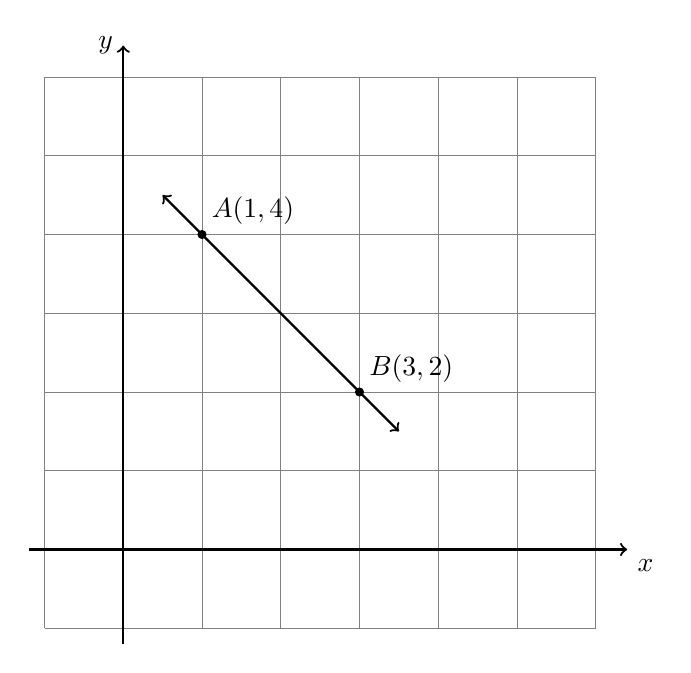
\begin{tikzpicture}[scale=1]
      \draw [help lines] (-1,-1) grid (6,6);
      \draw [thick, ->] (-1.2,0) -- (6.4,0) node [below right] {$x$};
      \draw [thick, ->] (0,-1.2)--(0,6.4) node [left] {$y$};
      \draw [fill] (1,4) circle [radius=0.05] node[above right] {$A(1,4)$};
      \draw [fill] (3,2) circle [radius=0.05] node[above right] {$B(3,2)$};
      \draw [<->, thick] (0.5,4.5)--(3.5,1.5);
    \end{tikzpicture}
    \end{flushright}
\end{multicols}

\newpage
\item Plot the points and find the slope of the line $\overleftrightarrow{RS}$, $R(3,1)$, $S(5,5)$. Use the formula and show the substitution step. As a check, draw the line and count the rise and run.
\begin{multicols}{2}
  $\displaystyle m = \frac{y_S - y_R}{x_S - x_R}$
    \vspace{2cm}
    \begin{flushright}
    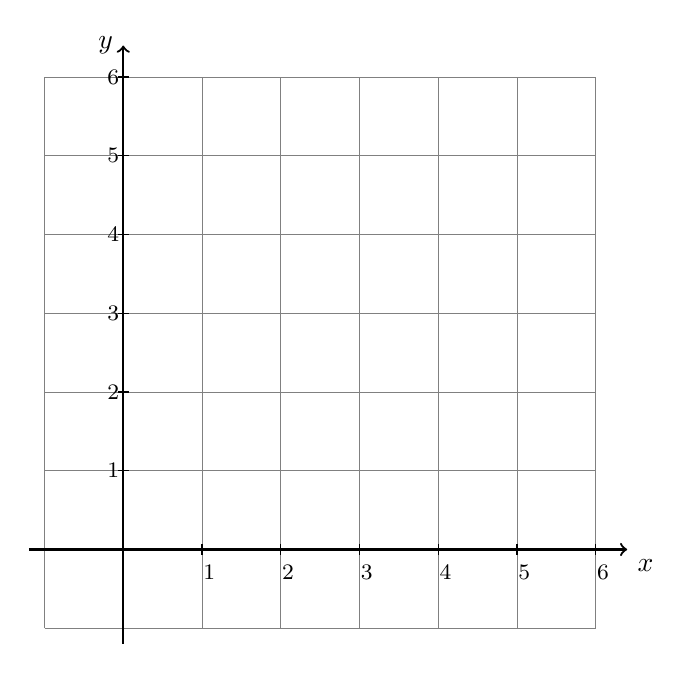
\begin{tikzpicture}[scale=1]
      \draw [help lines] (-1,-1) grid (6,6);
      \draw [thick, ->] (-1.2,0) -- (6.4,0) node [below right] {$x$};
      \foreach \x in {1,2,3,4,5,6}
        \draw[shift={(\x,0)},color=black] (0pt,2pt) -- (0pt,-2pt) node[below] {\footnotesize \; $\x$};
      \draw [thick, ->] (0,-1.2)--(0,6.4) node [left] {$y$};
      \foreach \y in {1,2,3,4,5,6}
        \draw[shift={(0,\y)},color=black] (-2pt,0pt) -- (2pt,0pt) node[left] {\footnotesize \; $\y$};
      %\draw [fill] (2,1) circle [radius=0.05] node[above left] {$A(2,1)$};
      %\draw [fill] (3,4) circle [radius=0.05] node[above right] {$B(3,4)$};
      %\draw [<->, thick] (1,-2)--(4,7);
    \end{tikzpicture}
    \end{flushright}
\end{multicols}

\newpage
\item Find the equation of the given line $\overleftrightarrow{AB}$, $A(0,1)$, $B(6,3)$.
\begin{multicols}{2}
    \begin{enumerate}[itemsep=1.2cm]
      \item Find the slope, $m$, showing the substitution step in the slope formula: \\[0.25cm]
      $\displaystyle m = (y_B - y_A)/(x_B - x_A)$
      \item Write down the $y$-intercept.
      \item Write the equation of the line.
      \end{enumerate}
    \begin{flushright}
    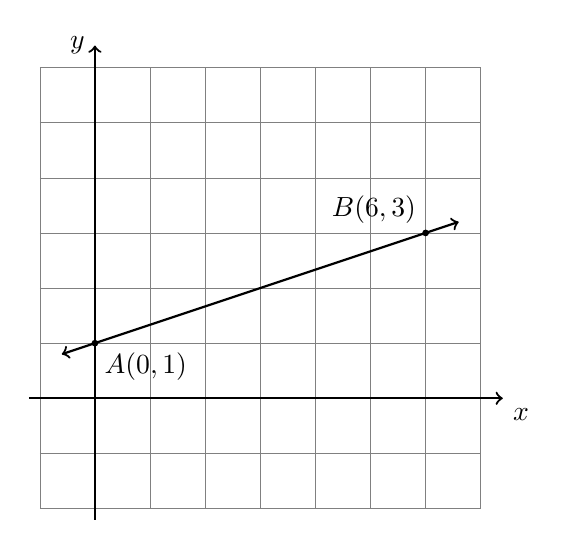
\begin{tikzpicture}[scale=0.7]
      \draw [help lines] (-1,-2) grid (7,6);
      \draw [thick, ->] (-1.2,0) -- (7.4,0) node [below right] {$x$};
      \draw [thick, ->] (0,-2.2)--(0,6.4) node [left] {$y$};
      \draw [fill] (0,1) circle [radius=0.05] node[below right] {$A(0,1)$};
      \draw [fill] (6,3) circle [radius=0.05] node[above left] {$B(6,3)$};
      \draw [<->, thick] (-0.6,0.8)--(6.6,3.2);
    \end{tikzpicture}
    \end{flushright}
\end{multicols}

\newpage
\item Complete each statement about linear equations.
\begin{enumerate}[itemsep=0.5cm]
  \item What is the $y$-intercept of the line $y = 3x - 1$?
  \item What is the slope of the line $y = x + 13$?
  \item Which has an undefined slope, a vertical or horizontal line?
  \item What is the $y$-intercept of the line $y = \frac{5}{2}x$?
  \item What is the slope of a horizontal line?

\end{enumerate}

\newpage
\item Is the point $C(6,5)$ on the line $l: y=\frac{1}{2}x+2$? \\[0.5cm]
Support your answer with \emph{both} algebra (substitute $C$'s coordinates into the equation) and geometry by graphing the line and point $C$.
  \begin{flushright}
  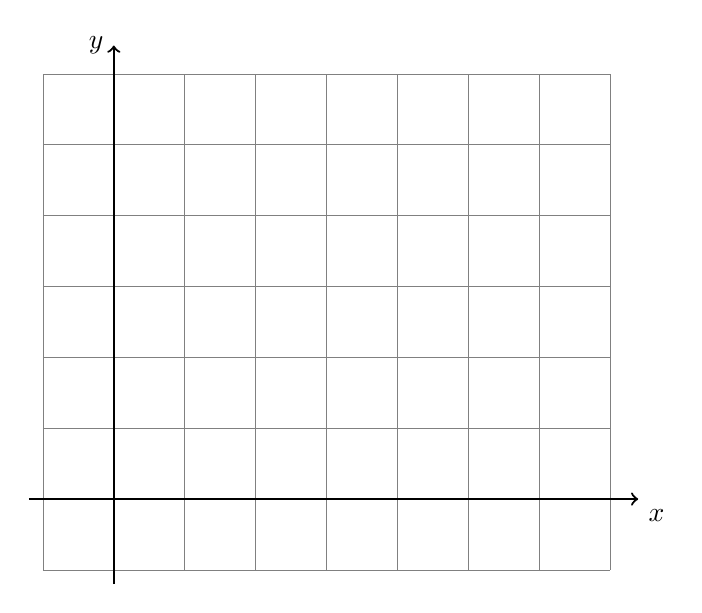
\begin{tikzpicture}[scale=0.9]
    \draw [help lines] (-1,-1) grid (7,6);
    \draw [thick, ->] (-1.2,0) -- (7.4,0) node [below right] {$x$};
    \draw [thick, ->] (0,-1.2)--(0,6.4) node [left] {$y$};
  \end{tikzpicture}
  \end{flushright}

\newpage
\item Write down the slope perpendicular to each slope (its negative reciprocal).
  \begin{enumerate}[itemsep=0.9cm]
    \item If $m = -5$ then $m_{\perp}=$
    \item If $\displaystyle m = \frac{3}{4}$ then $m_{\perp}=$
    \item If $m = -1$ then $m_{\perp}=$
    \item If $\displaystyle m = \frac{1}{7}$ then $m_{\perp}=$
  \end{enumerate}
  
\newpage
\item Two perpendicular lines are shown in the graph, $p$ and $q$. Line $p$ has a slope of $\displaystyle m = -\frac{1}{2}$ and a $y$-intercept $b=5$.
\begin{multicols}{2}
    \begin{enumerate}[itemsep=1cm]
      \item Write down the equation of line $p$.
      \item What is the slope of line $q$, $m_\perp$?
      \item Spicy: Line $q$ crosses the $x$-axis at $(5,0)$. What is its $y$-intercept?
      \end{enumerate}
    \begin{flushright}
    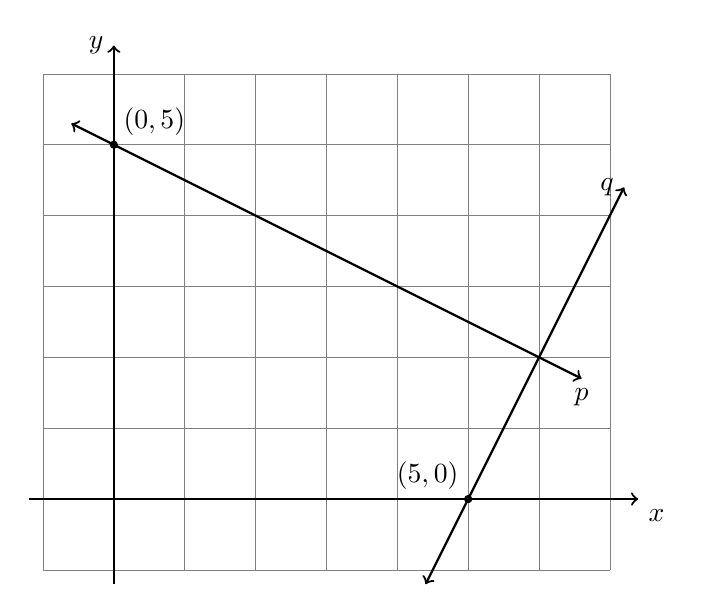
\begin{tikzpicture}[scale=0.9]
      \draw [help lines] (-1,-1) grid (7,6);
      \draw [thick, ->] (-1.2,0) -- (7.4,0) node [below right] {$x$};
      \draw [thick, ->] (0,-1.2)--(0,6.4) node [left] {$y$};
      \draw [fill] (0,5) circle [radius=0.05] node[above right] {$(0,5)$};
      \draw [fill] (5,0) circle [radius=0.05] node[above left] {$(5,0)$};
      \draw [<->, thick] (-0.6,5.3)--(6.6,1.7) node [below]{$p$};
      \draw [<->, thick] (4.4,-1.2)--(7.2,4.4) node [left]{$q$};
    \end{tikzpicture}
    \end{flushright}
\end{multicols}

\newpage
\item $\triangle ABC$ with vertices $A(2,5)$, $B(4,1)$, and $C(1,-1)$ is shown. \\[0.5cm]
Find the slopes of $\overleftrightarrow{AC}$ and $\overleftrightarrow{BC}$. Is the triangle a right triangle? Justify your answer.
  \begin{flushright}
    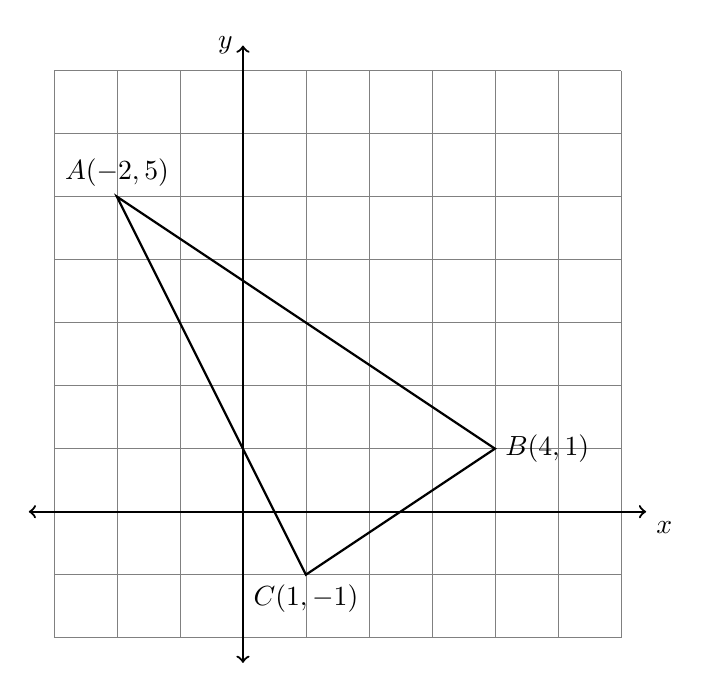
\begin{tikzpicture}[scale=0.8]
      \draw [help lines] (-3,-2) grid (6,7);
      \draw [thick, <->] (-3.4,0) -- (6.4,0) node [below right] {$x$};
      \draw [thick, <->] (0,-2.4)--(0,7.4) node [left] {$y$};
      \draw [thick] (-2,5) node[above] {$A(-2,5)$}--
        (1,-1) node[below] {$C(1,-1)$}--
        (4,1) node[right] {$B(4,1)$}--
        cycle;
    \end{tikzpicture}
    \end{flushright}

\newpage
\item Plot a right triangle using Geogebra (use the grid). The legs must not be horizontal or vertical. Paste an image of your work in this Classkick slide from the clipboard or by using the ``camera'' tool.\\[0.25cm]
Spicy: Show the measures the slopes of the triangle legs and the measure of the right angle.

    
\end{enumerate}
\end{document}

\newpage
\item A point labeled $C$ and vector $(1,3)$ are shown Geogebra/classic. Identify the following objects and tools.
  \begin{enumerate}
    \item Circle the vector
    \item Make an ``X'' where to click for the menu ``Name \& Value'' that will label point $C$ as an ordered pair.
    \item Mark with an arrow the menu where the ``Translate by vector'' tool is found.
  \end{enumerate}
  \begin{flushright}
    \includegraphics[width=6in]{5-11Geogebra_toolbar.png}
  \end{flushright}
